\documentclass[12pt]{scrreprt}

\usepackage[utf8]{inputenc}		% Ermögicht es umlaute direkt zu schreiben
\usepackage{amsmath,amssymb} 	% Mathe symbole und funktionen
\usepackage{graphicx}			% Bilder einbinden
\usepackage[ngerman]{babel} 	% Deutscht alles ein
\usepackage{pdflscape}			% Querformat
\usepackage[section]{placeins}	% Verhindert das Gleiten von Bildern in andere Sections

\parindent 0px					% Einrückung von absätzen auf 0

\subject{Teilentwurf}
\title{LISE E-Learning System}
\author{Matthias Englert, Fabian Schilha, Andreas Rottach}
\date{Wintersemester 2014/2015}

\begin{document}
\maketitle

\tableofcontents


\chapter{Datenbankentwurf}

\section{Datebankdiagramm}
\begin{figure}[h]
	\centering
	\paragraph{Aufbau der Relationalen Datenbank}	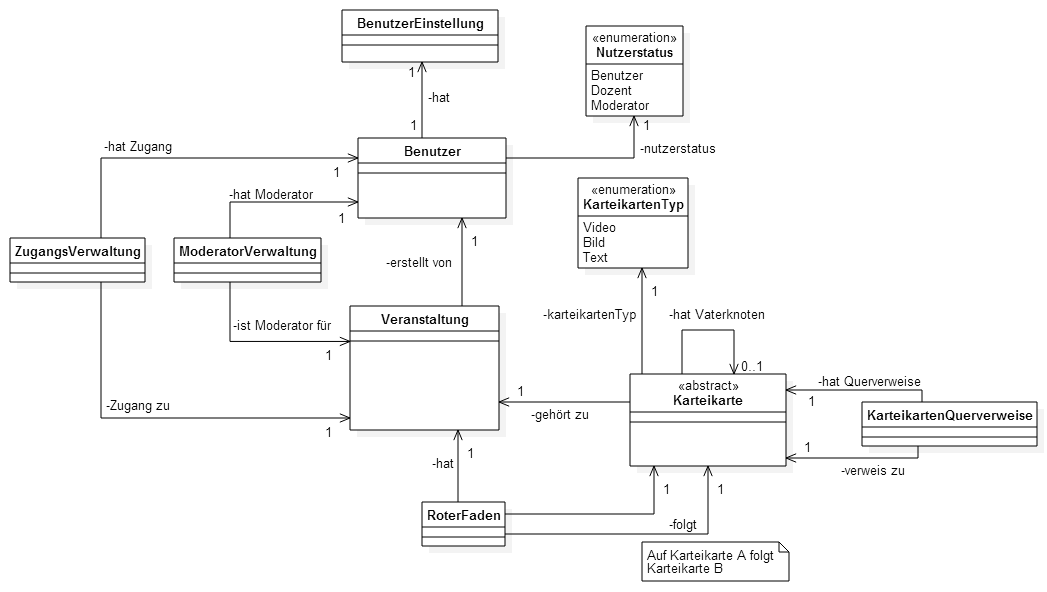
\includegraphics[width=\textwidth]{Bilder/Datenbank/Datenbankentwurf.png}
	\caption{Datenbankdiagramm}
	\label{Datenbankdiagramm}
\end{figure}

\section{Beschreibung der Tabellen}

\begin{tabular}{|lp{12cm}|}
	\hline
	TABELLE			&  Benutzer\\ 
	BESCHREIBUNG	&  Speichert alle Informationen, die zu einem Benutzer gehören.\\ 
	VERWALTET		& Benutzerdaten\\ 
	SCHLÜSSEL		&  ID : Integer\\ 
	\hline
	&  \\ 
	FELD		    &  Vorname : String\\  
	&  \\ 
	FELD		    &  Nachname : String\\  
	&  \\ 
	FELD		    &  Martrikelnummer : Integer\\  
	&  \\
	FELD		    &  eMail : String\\ 
	BESCHREIBUNG	&  Veranstaltungsbeschreibung\\
	&  \\
	FELD		    &  Studiengang : Enum\\ 
	BESCHREIBUNG	&  Fremdschlüssel, Benutzer ist bestimmtem Studiengang zugeordnet. Dozenten sind hier keinem Studiengang zugeordnet. Referenziert auf Tabelle Studiengang\\ 
	&  \\
	FELD		    &  Kennwport : String\\ 
	BESCHREIBUNG	&  Speichert das verschlüsselte Passwort des Nutzers \\
	&  \\
	FELD		    &  Nutzerstatus : Enum\\ 
	BESCHREIBUNG	&  Speichert ob Benutzer ein Student oder Dozent ist.\\
	&  \\
	FELD		    &  GruppeneinladungenErlauben : Bool\\ 
	BESCHREIBUNG	&  Speichert ob Benutzer zu Gruppen eingeladen werden kann.\\
	&  \\
	FELD		    &  NotifyDiskussionen : Enum\\ 
	BESCHREIBUNG	&  Speichert wie ein Benutzer über Diskussionen informiert wird.\\
	\hline
\end{tabular}\\\\

\begin{tabular}{|lp{12cm}|}
	\hline
	TABELLE			&  Studiengang\\ 
	BESCHREIBUNG	&  alle Studiengänge an der Universität Ulm\\ 
	VERWALTET		&  Benutzer und deren eingetragenen Studiengang\\ 
	SCHLÜSSEL		&  ID : Integer\\ 
	\hline
	&  \\
	FELD		    &  Studiengang : String\\ 
	BESCHREIBUNG	&  Text der den Studiengang beschreibt.\\
	\hline
\end{tabular}\\\\


\chapter{System-Architektur}
\section{Kommunikationsdiagramme}
\begin{figure}[h]
	\centering
	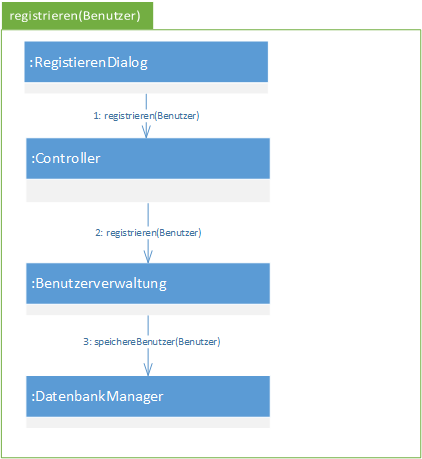
\includegraphics[width=0.7\linewidth]{Bilder/Kommunikationsdiagramme/registrieren}
	\caption{Registrierung}
	\label{Registrierung}
\end{figure}

\begin{figure}[h]
\centering
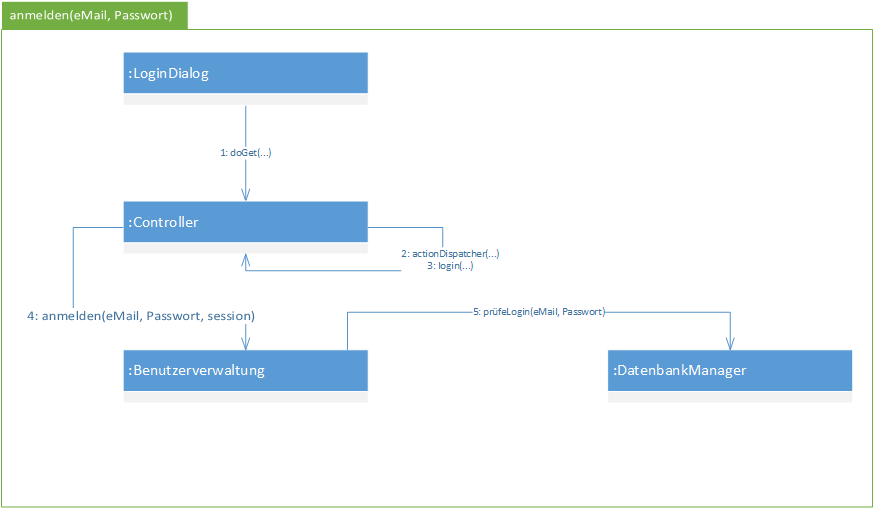
\includegraphics[width=\linewidth]{Bilder/Kommunikationsdiagramme/anmelden}
\caption{Am System anmelden}
\label{Am System anmelden}
\end{figure}

\begin{figure}[h]
\centering
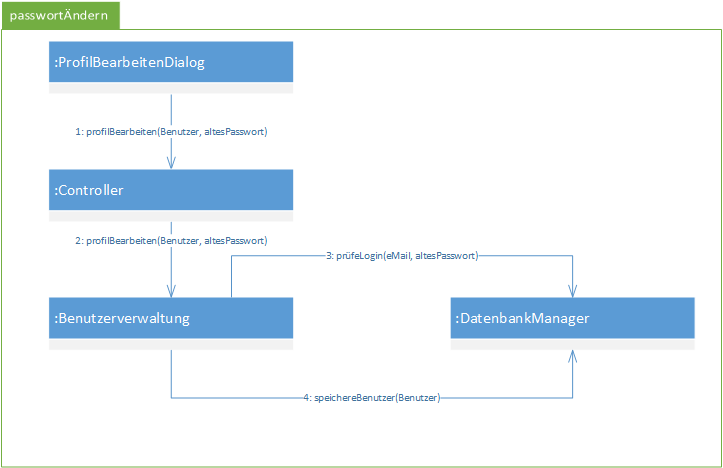
\includegraphics[width=\linewidth]{Bilder/Kommunikationsdiagramme/passwortAendern}
\caption{Passwortänderung}
\label{Passwortaenderung}
\end{figure}

\begin{landscape}
\section{Klassendiagramm}
\begin{figure}[!h]
\centering
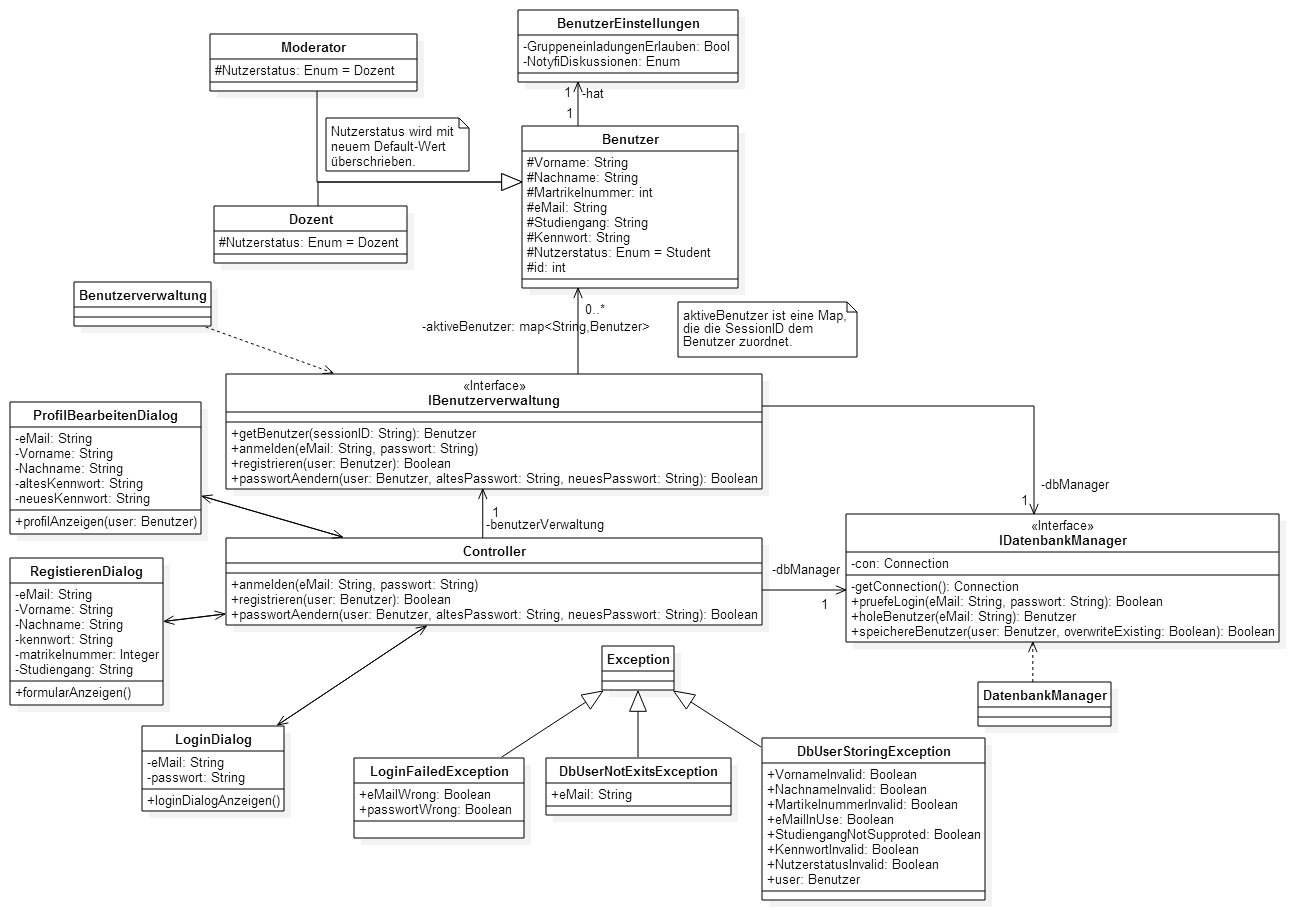
\includegraphics[width=\textwidth]{Bilder/Klassendiagramm/Klassendiagramm}
\caption{Klassendiagramm mit Realisierungsklassen}
\label{fig:Klassendiagramm}
\end{figure}
\end{landscape}

\section{Methodenbeschreibung}
\subsection{Controller Methoden}

\begin{tabular}{|lp{12cm}|}
	\hline
	Operation &  \textbf{doGet(HttpServletRequest request, HttpServletResponse response)}\\ 
	Beschreibung & Diese Methode nimmt einen Ankommenden Request entgegen und gibt ihn an die Methode "actinDispatcher" weiter. \\ 
	\hline 
\end{tabular} \\\\

\begin{tabular}{|lp{12cm}|}
	\hline
	Operation &  \textbf{actionDispatcher(HttpServletRequest request, HttpServletResponse response, HttpSession session)}\\ 
	Beschreibung & Diese Methode verwaltet die Weiterleitung zu den jeweils verantwortlichen Methoden für die Verarbeitung der Anfragen oder sie leitet weiter zu den Dialogen. \\ 
	\hline 
\end{tabular} \\\\

\begin{tabular}{|lp{12cm}|}
	\hline
	Operation &  \textbf{aenderePasswort(HttpServletRequest request, HttpServletResponse response, HttpSession session) }\\ 
	Beschreibung & Diese Methode übernimmt die Verarbeitung der Passwort-Änderungs-Anfragen Sie liest die Parameter aus dem Request aus. Wenn diese richtig angegeben sind wird die Anfrage an die Benutzerverwaltung weitergegeben. Je nachdem ob dies erfolgreich war, wird dann auf die Seite weitergeleitet oder der Benutzer landet wieder beim gleichen Dialog, wenn ein Fehler auftrat.\\ 
	\hline 
\end{tabular} \\\\
	
\begin{tabular}{|lp{12cm}|}
	\hline
	Operation &  \textbf{login(HttpServletRequest request, HttpServletResponse response, HttpSession session)}\\ 
	Beschreibung & Diese Methode übernimmt die Login-Anfragen. Sie liest die Parameter aus und leitet die Anfrage an die Benutzerverwaltung weiter. Es wird entweder auf die Startseite oder wieder die Loginseite weitergeleitet. \\ 
	\hline 
\end{tabular} \\\\

\begin{tabular}{|lp{12cm}|}
	\hline
	Operation &  \textbf{logout(HttpServletRequest request, HttpServletResponse response, HttpSession session)}\\ 
	Beschreibung & Diese Methode übernimmt die Logout-Anfragen. Sie liest die Parameter aus und leitet die Anfrage an die Benutzerverwaltung weiter. Es wird auf die Loginseite weitergeleitet. \\ 
	\hline 
\end{tabular} \\\\

\begin{tabular}{|lp{12cm}|}
	\hline
	Operation &  \textbf{registrieren(HttpServletRequest request, HttpServletResponse response)}\\ 
	Beschreibung & Diese Methode übernimmt die Registrierungsanfragen. Sie liest die Parameter aus und leitet die Anfrage an die Benutzerverwaltung weiter. Es wird auf die Loginseite weitergeleitet. \\ 
	\hline 
\end{tabular} \\\\

\begin{tabular}{|lp{12cm}|}
	\hline
	Operation &  \textbf{userValid(Benutzer b, HttpServletRequest request): Boolean}\\ 
	Beschreibung & Diese Methode prüft, ob die gespeicherten Benutzerdaten gültig sind. Sie prüft ob alle Werte gesetzt sind und ob die eMail bspw. ein \@ und einen Punkt enthält. \\ 
	\hline 
\end{tabular} \\\\

\begin{tabular}{|lp{12cm}|}
	\hline
	Operation &  \textbf{isEmpty(String s)}\\ 
	Beschreibung & Diese Methode prüft, ob der übergeben String null ist oder ob es ein Leerstring ist. \\ 
	\hline 
\end{tabular} \\\\

\subsection{Benutzerverwaltung  Methoden}

\begin{tabular}{|lp{12cm}|}
	\hline
	Operation &  \textbf{getBenutzer(HttpSession: session): Benutzer) }\\ 
	Beschreibung & Liefert das Benutzerobjekt zur entsprechenden Session zurück. Wenn die eMail-Addresse in der Session gespeichert ist, ist der Benutzer angemeldet. Dann wird das komplette Benutzerobjekt mit Hilfe des DB-Managers geladen und zurückgeliefert. Wenn ein Fehler auftritt wird null zurückgegeben.\\
	\hline 
\end{tabular} \\\\


\begin{tabular}{|lp{12cm}|}
	\hline
	Operation &  \textbf{anmelden(eMail:String, passwort:String, HttpSession: session) }\\ 
	Beschreibung & Meldet den Benutzer mit Passwort und eMail im System an. Die eMail wird in der aktuellen Session gespeichert um einen Verweis auf den Benutzer zu haben. \\ 
	\hline 
\end{tabular} \\\\

\begin{tabular}{|lp{12cm}|}
	\hline
	Operation &  \textbf{registrieren(user:Benutzer): Boolean) }\\ 
	Beschreibung & Ruft beim Datenbankmanager "speichereBenutzer" auf. Wenn user null ist wird eine NullPointerException geworfen. \\ 
	\hline 
\end{tabular} \\\\

\begin{tabular}{|lp{12cm}|}
	\hline
	Operation &  \textbf{passwortAendern(HttpSession session, altesPasswort:String, neuesPasswort:String): Boolean }\\ 
	Beschreibung & Diese Methode ändert das Passwort für den aktuell angemeldeten Benutzer, indem es den aktuellen Benutzer mit "holeBenutzer" holt, das Passwort neu setzt und den Benutzer mit Hilfe des Datenbankmanagers mit "bearbeiteBenutzer" speichert.\\ 
	\hline 
\end{tabular} \\\\

\begin{tabular}{|lp{12cm}|}
	\hline
	Operation &  \textbf{abmelden(HttpSession session): Boolean }\\ 
	Beschreibung & Falls ein Benutzer in der übergebenen Session angemeldet ist, wird die eMail aus der Session entfernt und der Benutzer somit abgemeldet. Ist der Benutzer schon ausgeloggt wird einfach false zurückgegeben.\\ 
	\hline 
\end{tabular} \\\\

\begin{tabular}{|lp{12cm}|}
	\hline
	Operation &  \textbf{istEingeloggt(HttpSession session): Boolean }\\ 
	Beschreibung & Prüft ob die eMail in der aktuellen Session enthalten ist. Wenn dies zutrifft ist der Benutzer angemeldet.\\ 
	\hline 
\end{tabular} \\\\


\subsection{Datenbankmanager  Methoden}
\begin{tabular}{|lp{12cm}|}
	\hline
	Operation &  \textbf{getConnection(): Connection}\\ 
	Beschreibung & Mit dieser Methode wird eine Verbindung zur Datenbank aufgebaut. Für alle Datenbankoperationen ist es eine Vorbedingung, dass eine Verbindung zur Datenbank existiert. \\ 
	\hline 
\end{tabular} \\\\

\begin{tabular}{|lp{12cm}|}
	\hline
	Operation &  \textbf{pruefeLogin(eMail:String, passwort:String): Boolean}\\ 
	Beschreibung & \\ Es wird geprüft ob es in der Datenbank einen Benutzer mit der übergebenen eMail Adresse gibt. Als zweiter Schritt prüft die Methode, ob das Passwort zu diesem Benutzer passt. Wenn nicht wirft die Operation eine LoginFailedException. Die Exception bekommt als Parameter angegeben, ob die eMail oder das Passwort fehlerhaft ist. Sind die Benutzerdaten in Ordnung, dann gibt die Methode true zurück, ansonsten false.
	\hline 
\end{tabular} \\\\

\begin{tabular}{|lp{12cm}|}
	\hline
	Operation &  \textbf{holeBenutzer(eMail:String): Benutzer}\\ 
	Beschreibung & \\ Vorbedingung: Benutzer in der Datenbank vorhanden. Die Operation liest aus der Datenbank den Benutzer mit der angegebenen eMail. Gibt es keinen passenden Benutzer in der Datenbank zu dieser eMail, dann wirft die Operation eine DbUserNotExistsException. Als Nachbedingung wird der Benutzer zurückgeliefert.
	\hline 
\end{tabular} \\\\

\begin{tabular}{|lp{12cm}|}
	\hline
	Operation &  \textbf{speichereBenutzer(user:Benutzer): Boolean}\\ 
	Beschreibung & \\ Vorbedingung: Attribute des Benutzers sind alle korrekt. Beispielsweise dürfen Name und Vorname keine Leerstrings sein oder die eMail des Benutzers muss eindeutig sein. Außerdem muss der Studiengang des Benutzers in der Datenbanktabelle Studiengang vorhanden sein. Die Operation speichert den Benutzer in der Datenbank in der Tabelle Benutzer. Nachbedingung ist dass der Benutzer in der Datenbank gespeichert ist.
	\hline 
	
	Operation &  \textbf{bearbeiteBenutzer(user:Benutzer)}\\ 
	Beschreibung & \\ Vorbedingung: Benutzer ist in der Datenbank vorhanden, die Attribute des Benutzers sind alle korrekt und der Studiengang des Benutzers in der Datenbanktabelle Studiengang vorhanden sein. Die Operation ändert die Attribute des Benutzers in der Datenbank.
	\hline 
	
	Operation &  \textbf{holeStudiengaenge(): List<String>}\\ 
	Beschreibung & \\ Es gibt keine Vorbedingungen. Die Operation liest alle Studiengänge aus der Datenbank aus und gibt sie in einer Liste zurück.
		\hline 
\end{tabular} \\\\


\subsection{RegistrierenDialog  Methoden}

\begin{tabular}{|lp{12cm}|}
	\hline
	Operation &  \textbf{formularAnzeigen()}\\ 
	Beschreibung & \\ 
	\hline 
\end{tabular} \\\\

\paragraph{LoginDialog  Methoden}\mbox{}\\

\begin{tabular}{|lp{12cm}|}
	\hline
	Operation &  \textbf{loginDialogAnzeigen()}\\ 
	Beschreibung & \\ 
	\hline 
\end{tabular} \\\\

\subsection{ProfilBearbeitenDialog  Methoden}

\begin{tabular}{|lp{12cm}|}
	\hline
	Operation &  \textbf{profilAnzeigen(user:Benutzer)}\\ 
	Beschreibung & \\ 
	\hline 
\end{tabular} \\\\

\end{document}
